%====================================================================
%====================================================================
\section*{Backup}
%====================================================================
\frame{\frametitle{Reparametrization trick} \label{goto:reparmTrick}

  Denoting by $\psi$ the variational parameter, The VE step aims at minimizing
  $$
  KL[q_\psi(Z) \| p_\theta(Z \mid Y)] = \Esp_{q_\psi} \log \frac{q_\psi(Z)}{p_\theta(Z \mid Y)}
  $$
  
  \bigskip 
  Stochastic gradient descent requires an unbiased estimate of the gradient $\nabla_\psi \Esp_{q_\psi} (\cdot)$ ... \\
  which is {\sl not} provided by sampling $Z^b \overset{\text{iid}}{\sim} q_\psi$ to estimate $\Esp_{q_\psi}$.

  \bigskip \bigskip 
  \paragraph{Trick \refer{KiW14,KiW19}.}
  Suppose there exist a fix distribution $q^0$ and a function $f$, such that\footnote{Think of $q^0 = \Ncal(0, I)$, $\psi = (\mu, \Sigma)$, $q_\psi = \Ncal(\mu, \Sigma)$.}
  $$
  \epsilon \sim q^0 
  \qquad \Rightarrow \qquad Z = f(\epsilon, \psi) \sim q_\psi, 
  $$
  Then, sampling $\epsilon^b \overset{\text{iid}}{\sim} q^0$ provides an unbiased estimate of the gradient:
  $$
  \nabla_\psi \; \Esp_{q_\psi} \log \frac{q_\psi(Z)}{p_\theta(Z \mid Y)}
  \simeq 
  \nabla_\psi \; \left( \frac1B \sum_b \log \frac{q_\psi(f(\epsilon^b, \psi))}{p_\theta(f(\epsilon^b, \psi) \mid Y)} \right)
  $$

  \textcolor{gray}{Back to \#\ref{back:reparmTrick}}

}

%====================================================================
\frame{\frametitle{VBEM for binary SBM}  \label{goto:vbemSBM}

  \paragraph{Posterio credibility intervals (CI) \refer{GDR12}:}  
  Actual level for $\pi_1$ ($+$), $\gamma_{11}$
  (\textcolor{red}{$\triangle$}), $\gamma_{12}$
  (\textcolor{blue}{$\circ$}), $\gamma_{22}$
  (\textcolor{green}{$\bullet$}) \\
  \includegraphics[width=.9\textwidth]{\fignet/im-ICQ2-2-new} \\
%   \pause \ra For all parameters, {\VBEM} posterior credibility
%   intervals achieve the nominal level (90\%), as soon as $n \geq 30$.

  \emphase{Width of the posterior CI.}
  {$\pi_1$}, \textcolor{red}{$\gamma_{11}$},
  \textcolor{blue}{$\gamma_{12}$}, \textcolor{green}{$\gamma_{22}$}
  \\
  \includegraphics[width=1\textwidth]{\fignet/im-ICQ2-3} \\

  \bigskip
  \ra 
  Width $\approx 1/\sqrt{n}$ for $\pi_1$ and $\approx 1/n = 1/\sqrt{n^2}$ for $\gamma_{11}$, $\gamma_{12}$ and $\gamma_{22}$.

  \bigskip
  \textcolor{gray}{Back to \#\ref{back:vbemSBM}}

}

%====================================================================
\frame{\frametitle{Largest gap algorithm} \label{goto:largestGap}

  \begin{tabular}{cc}
    \hspace{-.04\textwidth}
    \begin{tabular}{p{.45\textwidth}}
      \begin{itemize}
      \item \emphase{Degree} of a node: $D_i = \sum_{j \neq i} Y_{ij}$
      \item \bigskip Mean connection from group $k$:
      $$
      \overline{\gamma}_k = \sum_\ell \pi_\ell \gamma_{k\ell}
      $$
      \item \bigskip Degree distribution\footnote{Balanced affiliation model = nasty case: $\pi_k \equiv 1/K, \gamma_{kk} = \gamma_{in}, \gamma_{k\ell} = \gamma_{out} \quad \Rightarrow \quad  \overline{\gamma}_k \equiv (\gamma_{in} + (K-1)\gamma_{out})/K$}
      $$
      (D_i \mid Z_i = k) \sim \Bcal(n-1, \overline{\gamma}_k)
      $$
      \item \bigskip \emphase{Concentration} of $D_i / (n-1)$ around $\overline{\gamma}_{Z_i}$ at exponential rate 
      \end{itemize}
    \end{tabular}
    &
    \hspace{-.05\textwidth}
    \begin{tabular}{p{.45\textwidth}}
      \includegraphics[height=.7\textheight]{\fignet/FigLargestGap-Histograms}
    \end{tabular}
  \end{tabular}
  
  \ra Ensures consistency \refer{CDR12} (including sparse regime)  
  
  \bigskip
  \textcolor{gray}{Back to \#\ref{back:largestGap}}

}
  
%====================================================================
\frame{\frametitle{Sequential importance sampling scheme} \label{goto:SMC}

  Consider $\emphase{U = (\theta, Z)}$
  
  \bigskip
  \paragraph{Distribution path:}
    set $0 = \rho_0 < \rho_1 < \dots < \rho_{H-1} < \rho_H = 1$,
  \begin{align*}
     p_h(U) & \propto p_{\text{start}}(U)^{\emphase{{1-\rho_h}}} \; \times \; p_{\text{target}}(U)^{\emphase{{\rho_h}}} \\
     \\
     & \propto p_{\text{start}}(U) \; \times \; r(U)^{\emphase{{\rho_h}}}, 
     & r(U) & = \frac{p(U) p(Y \mid U)}{p_{\text{start}}(U)}
  \end{align*}
  
  \bigskip \bigskip \pause
  \paragraph{Sequential sampling.} At each step $h$, provides
  $$
  \Ecal_h = \{(U_h^m, w_h^m)\}_m = \text{ weighted sample of } p_h
  $$

  \bigskip \pause
  \paragraph{Tune $\rho_{h+1}$} 
  to keep the efficient sample size sufficiently high at each step. \\
  ~ \\
  \ra Doable because $r(U)$ does not depend on $\rho$.

}

%====================================================================
\frame{\frametitle{Sequential sampling: in pictures}  

  \begin{tabular}{cc}
    \hspace{-.04\textwidth}
   \begin{tabular}{p{.5\textwidth}}
      \begin{itemize}
        \onslide+<1->{\item $\textcolor{blue}{p_{\text{start}}} = $ proposal, $\textcolor{red}{p_{\text{target}}} = $ target \\ ~ \\} 
        \onslide+<2->{\item Intermediate distributions
        $p_{\text{start}} = p_0$, $p_1$, $...$, $p_H = p_{\text{target}}$ \\ ~ \\}
        \onslide+<3->{\item Iteratively: \\
        use $p_h$ to get a sample from $p_{h+1}$}
      \end{itemize}
    \end{tabular}
    & 
    \hspace{-.02\textwidth}
    \begin{tabular}{p{.5\textwidth}}
      \begin{overprint}
        \onslide<1> 
        \includegraphics[width=.4\textwidth]{\figbayes/FigVBEM-IS-PropTarget-4to2}
        \onslide<2> 
        \includegraphics[width=.4\textwidth]{\figbayes/FigVBEM-IS-Tempering-4to2}
        \onslide<3> 
        \includegraphics[width=.4\textwidth]{\figbayes/FigVBEM-IS-Tempering-step1-4to2}
        \onslide<4> 
        \includegraphics[width=.4\textwidth]{\figbayes/FigVBEM-IS-Tempering-step2-4to2}
        \onslide<5> 
        \includegraphics[width=.4\textwidth]{\figbayes/FigVBEM-IS-Tempering-step3-4to2}
        \onslide<6-> 
        \includegraphics[width=.4\textwidth]{\figbayes/FigVBEM-IS-Tempering-step4-4to2}
      \end{overprint}
    \end{tabular}
  \end{tabular}  
  
  \bigskip
  \onslide+<7>{+ resampling/propagation to avoid complete degeneracy \refer{DoR19}}

  \bigskip
  \textcolor{gray}{Back to \#\ref{back:SMC}}

}

%====================================================================
\frame{\frametitle{Residual 'graphon'} \label{goto:graphon}

  \paragraph{Graphon representation of $(\pi, \alpha)$.} \refer{LaR16,DoR19}
  \begin{align*}
    \phi_K: (0, 1) \times (0, 1) \mapsto \Rbb
    \qquad \text{block wise constant} 
  \end{align*}
  For a given set $S$, averaging over $K$ gives
  $$
  \widehat{\phi}(u, v) 
  = \Esp \left(\phi_K(u, v) \mid Y, S\right)
  = \sum_K p(K \mid Y, S) \Esp \left(\phi_K(u, v) \mid Y, S, K\right)
  $$

  \pause \bigskip \bigskip
  $$
  \begin{array}{ccc}
    \text{SBM graphon} & \text{$\widehat{\phi}$ for the tree network} & \text{$U_i$ vs nb. neighbors} \\
    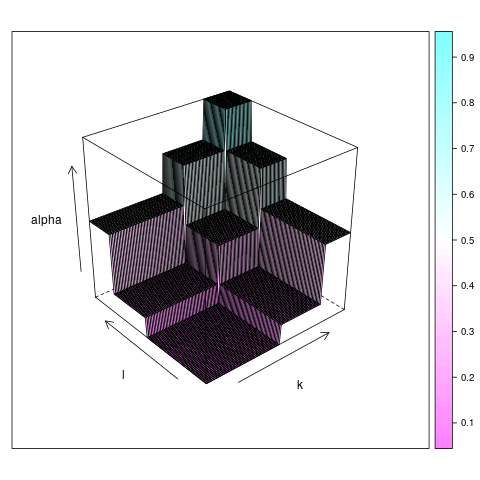
\includegraphics[trim=60 60 60 60, width=.25\textwidth]{\figDoR/FigGraphon-SBM-graphon-alpha} &
    \includegraphics[trim=60 60 60 60, width=.25\textwidth]{\figDoR/Tree-all-V10-M5000-graphon} &
    \includegraphics[width=.25\textwidth]{\figDoR/Tree-all-V10-M5000-Ui-neighbours} 
  \end{array}
  $$
  
  \bigskip
  \textcolor{gray}{Back to \#\ref{back:graphon}}
  
}

%====================================================================
\frame{\frametitle{SMC path} \label{goto:smcPath}

  $$
  \begin{array}{cc|c}
    \multicolumn{2}{c|}{\text{Tree network, $S = \{taxo., geo.\}$}}
    &  \text{Simulations} \\
    & & \\
    \hline
    \includegraphics[width=.25\textwidth]{\figDoR/Tree-all-V10-M5000-rho} & 
    \includegraphics[width=.25\textwidth]{\figDoR/Tree-all-V10-M5000-MI} &
    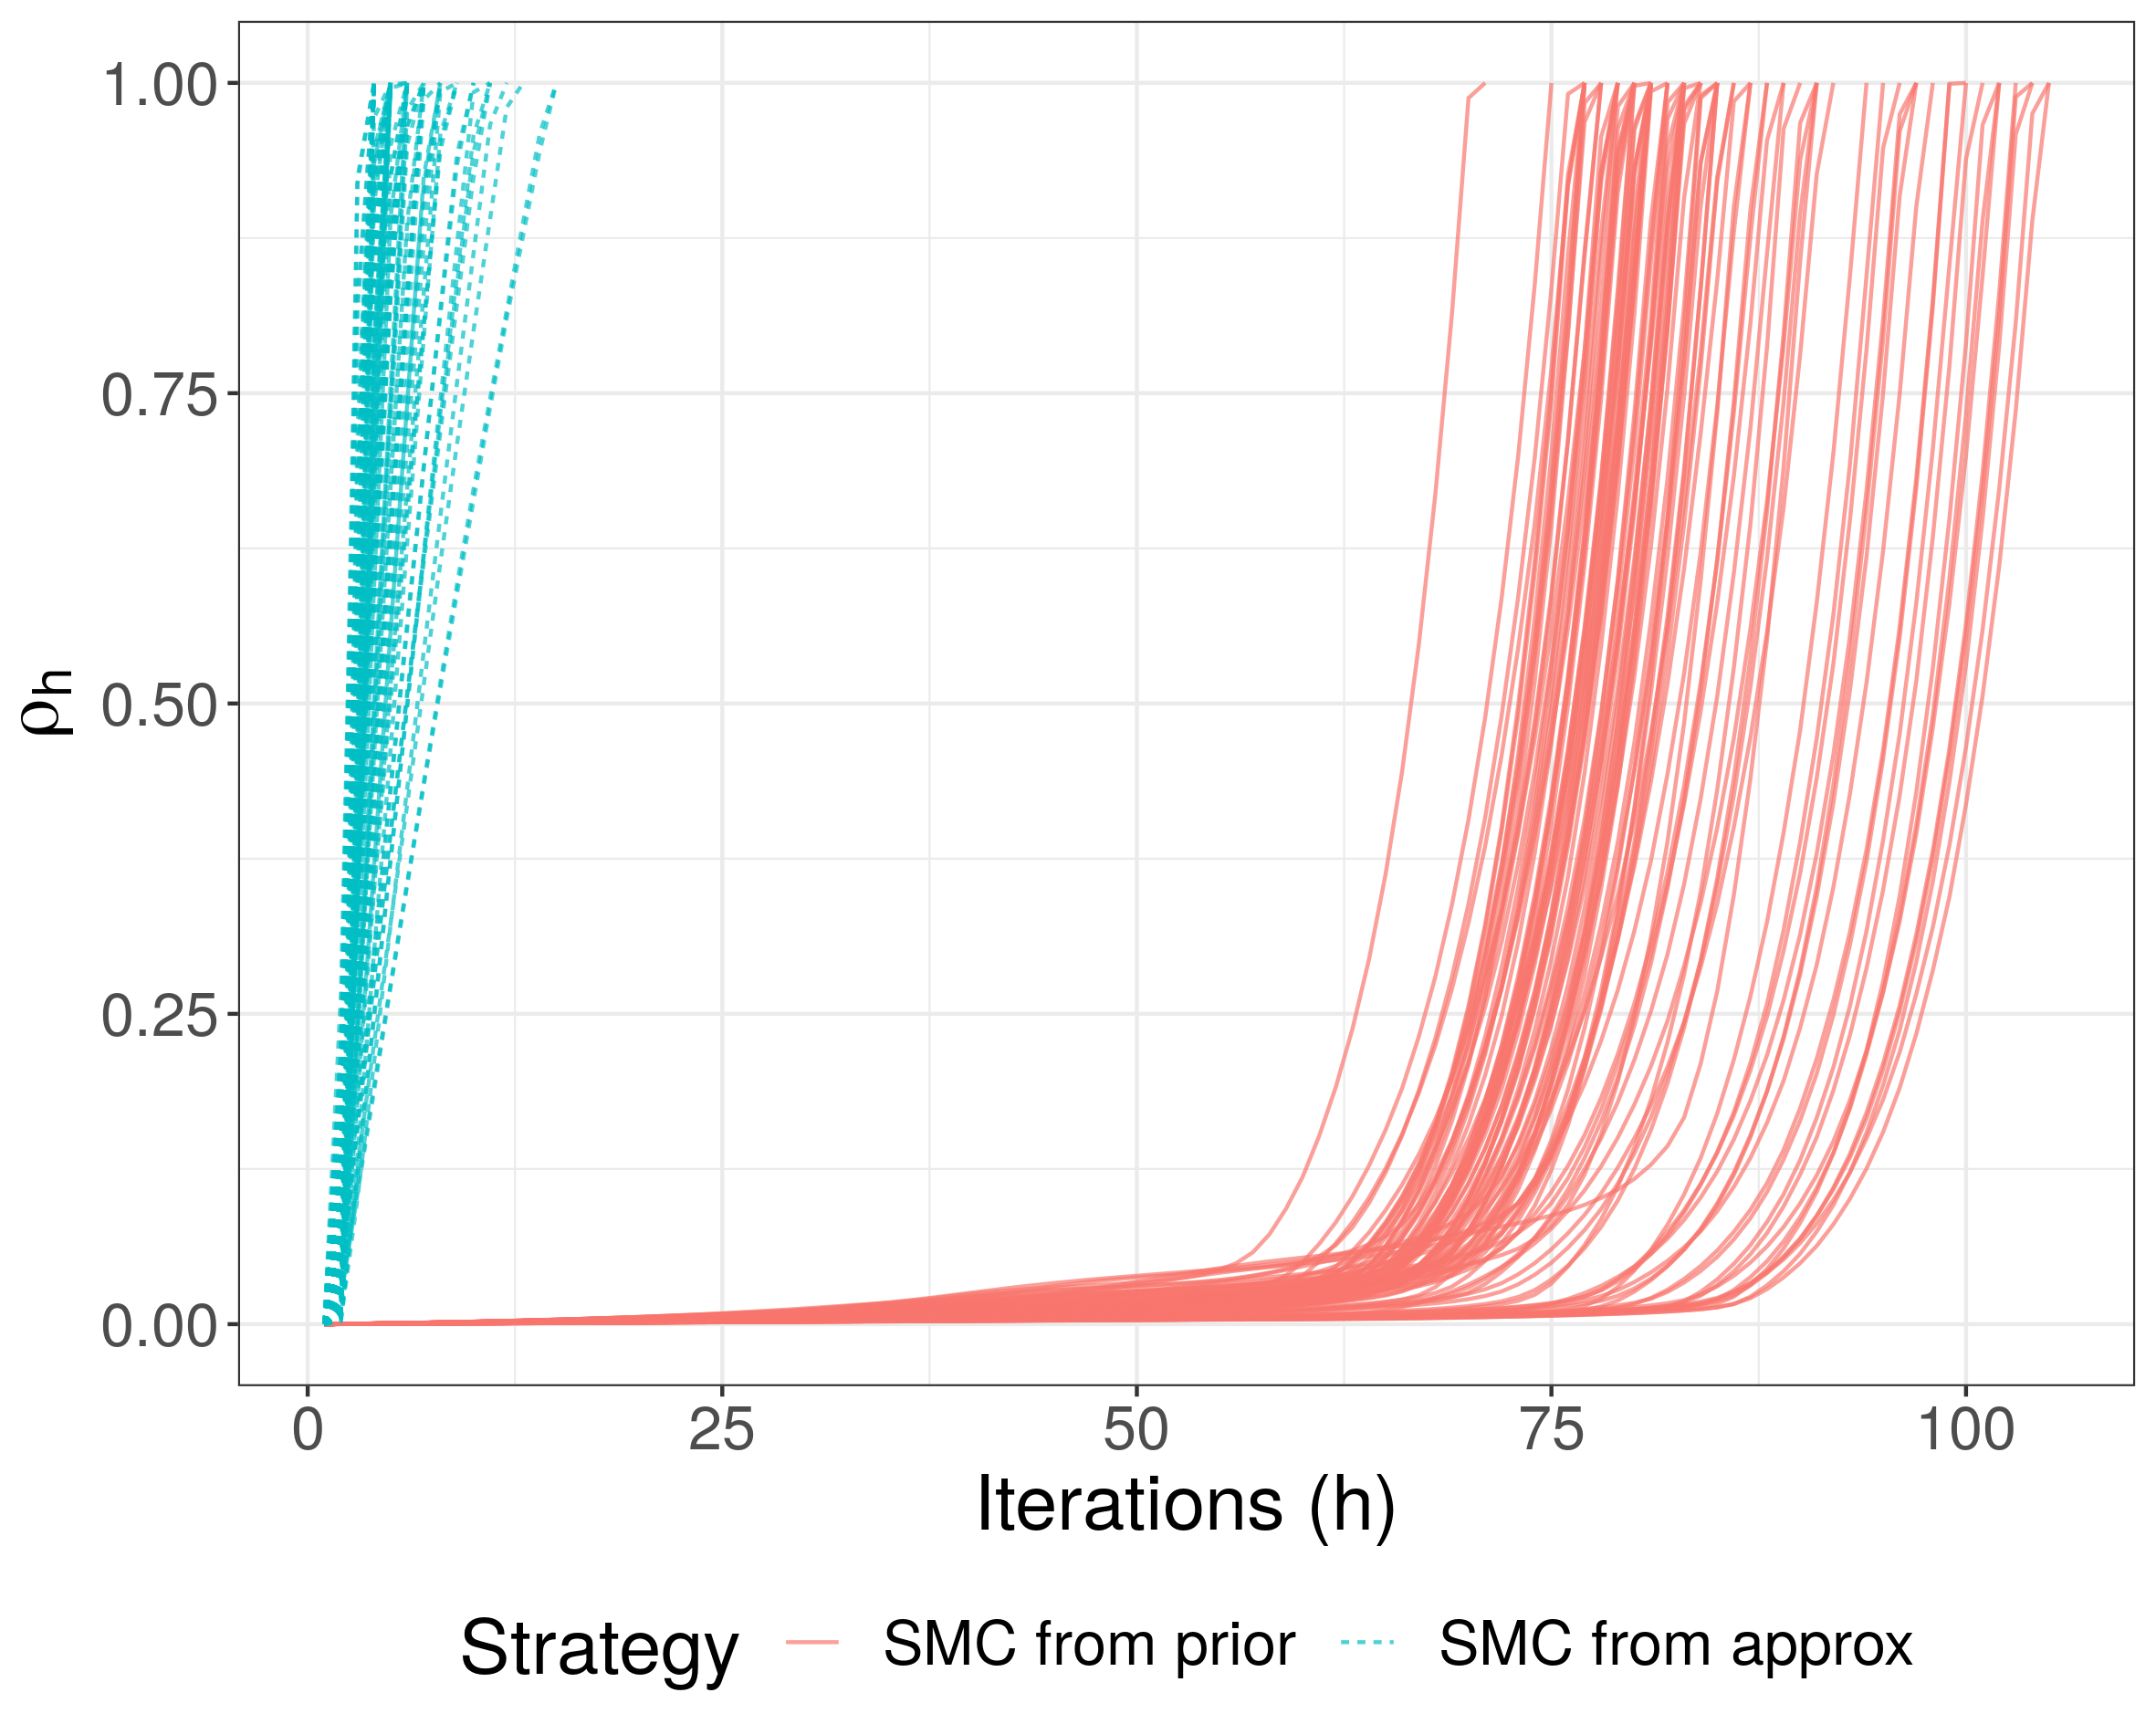
\includegraphics[width=.25\textwidth, height=.21\textwidth, trim=0 20 0 30]{\figDoR/simu_traj_rho} \\
    \rho_h 
    & \displaystyle{KL\left(p_h(Z) \; \| \; \prod_i p_h(Z_i)\right)} 
    & \\
  \end{array}
  $$
  from \refer{DoR19}
  
  \bigskip
  \textcolor{gray}{Back to \#\ref{back:smcPath}}
  
}

